% Options for packages loaded elsewhere
\PassOptionsToPackage{unicode}{hyperref}
\PassOptionsToPackage{hyphens}{url}
%
\documentclass[
]{article}
\usepackage{lmodern}
\usepackage{amssymb,amsmath}
\usepackage{ifxetex,ifluatex}
\ifnum 0\ifxetex 1\fi\ifluatex 1\fi=0 % if pdftex
  \usepackage[T1]{fontenc}
  \usepackage[utf8]{inputenc}
  \usepackage{textcomp} % provide euro and other symbols
\else % if luatex or xetex
  \usepackage{unicode-math}
  \defaultfontfeatures{Scale=MatchLowercase}
  \defaultfontfeatures[\rmfamily]{Ligatures=TeX,Scale=1}
\fi
% Use upquote if available, for straight quotes in verbatim environments
\IfFileExists{upquote.sty}{\usepackage{upquote}}{}
\IfFileExists{microtype.sty}{% use microtype if available
  \usepackage[]{microtype}
  \UseMicrotypeSet[protrusion]{basicmath} % disable protrusion for tt fonts
}{}
\makeatletter
\@ifundefined{KOMAClassName}{% if non-KOMA class
  \IfFileExists{parskip.sty}{%
    \usepackage{parskip}
  }{% else
    \setlength{\parindent}{0pt}
    \setlength{\parskip}{6pt plus 2pt minus 1pt}}
}{% if KOMA class
  \KOMAoptions{parskip=half}}
\makeatother
\usepackage{xcolor}
\IfFileExists{xurl.sty}{\usepackage{xurl}}{} % add URL line breaks if available
\IfFileExists{bookmark.sty}{\usepackage{bookmark}}{\usepackage{hyperref}}
\hypersetup{
  hidelinks,
  pdfcreator={LaTeX via pandoc}}
\urlstyle{same} % disable monospaced font for URLs
\usepackage[margin=1in]{geometry}
\usepackage{color}
\usepackage{fancyvrb}
\newcommand{\VerbBar}{|}
\newcommand{\VERB}{\Verb[commandchars=\\\{\}]}
\DefineVerbatimEnvironment{Highlighting}{Verbatim}{commandchars=\\\{\}}
% Add ',fontsize=\small' for more characters per line
\usepackage{framed}
\definecolor{shadecolor}{RGB}{248,248,248}
\newenvironment{Shaded}{\begin{snugshade}}{\end{snugshade}}
\newcommand{\AlertTok}[1]{\textcolor[rgb]{0.94,0.16,0.16}{#1}}
\newcommand{\AnnotationTok}[1]{\textcolor[rgb]{0.56,0.35,0.01}{\textbf{\textit{#1}}}}
\newcommand{\AttributeTok}[1]{\textcolor[rgb]{0.77,0.63,0.00}{#1}}
\newcommand{\BaseNTok}[1]{\textcolor[rgb]{0.00,0.00,0.81}{#1}}
\newcommand{\BuiltInTok}[1]{#1}
\newcommand{\CharTok}[1]{\textcolor[rgb]{0.31,0.60,0.02}{#1}}
\newcommand{\CommentTok}[1]{\textcolor[rgb]{0.56,0.35,0.01}{\textit{#1}}}
\newcommand{\CommentVarTok}[1]{\textcolor[rgb]{0.56,0.35,0.01}{\textbf{\textit{#1}}}}
\newcommand{\ConstantTok}[1]{\textcolor[rgb]{0.00,0.00,0.00}{#1}}
\newcommand{\ControlFlowTok}[1]{\textcolor[rgb]{0.13,0.29,0.53}{\textbf{#1}}}
\newcommand{\DataTypeTok}[1]{\textcolor[rgb]{0.13,0.29,0.53}{#1}}
\newcommand{\DecValTok}[1]{\textcolor[rgb]{0.00,0.00,0.81}{#1}}
\newcommand{\DocumentationTok}[1]{\textcolor[rgb]{0.56,0.35,0.01}{\textbf{\textit{#1}}}}
\newcommand{\ErrorTok}[1]{\textcolor[rgb]{0.64,0.00,0.00}{\textbf{#1}}}
\newcommand{\ExtensionTok}[1]{#1}
\newcommand{\FloatTok}[1]{\textcolor[rgb]{0.00,0.00,0.81}{#1}}
\newcommand{\FunctionTok}[1]{\textcolor[rgb]{0.00,0.00,0.00}{#1}}
\newcommand{\ImportTok}[1]{#1}
\newcommand{\InformationTok}[1]{\textcolor[rgb]{0.56,0.35,0.01}{\textbf{\textit{#1}}}}
\newcommand{\KeywordTok}[1]{\textcolor[rgb]{0.13,0.29,0.53}{\textbf{#1}}}
\newcommand{\NormalTok}[1]{#1}
\newcommand{\OperatorTok}[1]{\textcolor[rgb]{0.81,0.36,0.00}{\textbf{#1}}}
\newcommand{\OtherTok}[1]{\textcolor[rgb]{0.56,0.35,0.01}{#1}}
\newcommand{\PreprocessorTok}[1]{\textcolor[rgb]{0.56,0.35,0.01}{\textit{#1}}}
\newcommand{\RegionMarkerTok}[1]{#1}
\newcommand{\SpecialCharTok}[1]{\textcolor[rgb]{0.00,0.00,0.00}{#1}}
\newcommand{\SpecialStringTok}[1]{\textcolor[rgb]{0.31,0.60,0.02}{#1}}
\newcommand{\StringTok}[1]{\textcolor[rgb]{0.31,0.60,0.02}{#1}}
\newcommand{\VariableTok}[1]{\textcolor[rgb]{0.00,0.00,0.00}{#1}}
\newcommand{\VerbatimStringTok}[1]{\textcolor[rgb]{0.31,0.60,0.02}{#1}}
\newcommand{\WarningTok}[1]{\textcolor[rgb]{0.56,0.35,0.01}{\textbf{\textit{#1}}}}
\usepackage{graphicx,grffile}
\makeatletter
\def\maxwidth{\ifdim\Gin@nat@width>\linewidth\linewidth\else\Gin@nat@width\fi}
\def\maxheight{\ifdim\Gin@nat@height>\textheight\textheight\else\Gin@nat@height\fi}
\makeatother
% Scale images if necessary, so that they will not overflow the page
% margins by default, and it is still possible to overwrite the defaults
% using explicit options in \includegraphics[width, height, ...]{}
\setkeys{Gin}{width=\maxwidth,height=\maxheight,keepaspectratio}
% Set default figure placement to htbp
\makeatletter
\def\fps@figure{htbp}
\makeatother
\setlength{\emergencystretch}{3em} % prevent overfull lines
\providecommand{\tightlist}{%
  \setlength{\itemsep}{0pt}\setlength{\parskip}{0pt}}
\setcounter{secnumdepth}{-\maxdimen} % remove section numbering

\author{}
\date{\vspace{-2.5em}}

\begin{document}

\hypertarget{statistical-inference-course-project-simulation-and-inferential-data-analysis}{%
\section{Statistical Inference Course Project: Simulation and
Inferential Data
Analysis}\label{statistical-inference-course-project-simulation-and-inferential-data-analysis}}

\hypertarget{author-vin-lam}{%
\subsection{Author: Vin Lam}\label{author-vin-lam}}

\hypertarget{part-1-simulation-exercise}{%
\subsection{Part 1: Simulation
Exercise}\label{part-1-simulation-exercise}}

\hypertarget{overview}{%
\subsection{Overview:}\label{overview}}

In the first part of this exploration, we will examine the Law of Large
Numbers and the Central Limit Theorem being put to work in simulating
1000 exponential distributions with 40 draws each and a lambda of 0.2.
The goal is to show that these two important statistical properties
allow us to yield very good approximations for the mean and standard
deviation/variance of the true exponential distribution with lambda =
0.2. Not only very good approximations, but also that the distribution
is close to normal.

\hypertarget{sample-mean-and-theoretical-mean}{%
\subsection{Sample mean and theoretical
mean}\label{sample-mean-and-theoretical-mean}}

First let's calculate the theoretical mean of an exponential
distribution with lambda = 0.2. This is a very simple calculation,
because we know that the mean of an exponential distribution is 1/lambda
(as well as the standard deviation), which turns out to be exactly 5.

Now what about the sample mean? We will run 1000 simulations of
exponentials with 40 draws and lambda = 0.2 and calculate the mean for
every simulation. We will then take the average of all the means across
every simulation to obtain our sample mean.

\begin{Shaded}
\begin{Highlighting}[]
\NormalTok{mns =}\StringTok{ }\KeywordTok{c}\NormalTok{() }\CommentTok{#initialize mns to an empty vector}
\ControlFlowTok{for}\NormalTok{ (i }\ControlFlowTok{in} \DecValTok{1}\OperatorTok{:}\DecValTok{1000}\NormalTok{) }\CommentTok{# run 1000 simulations}
\NormalTok{  mns =}\StringTok{ }\KeywordTok{c}\NormalTok{(mns, }\KeywordTok{mean}\NormalTok{(}\KeywordTok{rexp}\NormalTok{(}\DecValTok{40}\NormalTok{,}\FloatTok{0.2}\NormalTok{))) }\CommentTok{# store the means of every simulation into mns}
\KeywordTok{mean}\NormalTok{(mns) }\CommentTok{# calculate the mean of mns, the sample mean}
\end{Highlighting}
\end{Shaded}

\begin{verbatim}
## [1] 5.026594
\end{verbatim}

As it turns out, the sample mean is an extremely close approximation of
the theoretical mean, 5. We can further show that with more draws
upwards to infinity, the sample mean converges to the theoretical.

\begin{Shaded}
\begin{Highlighting}[]
\KeywordTok{library}\NormalTok{(tidyverse)}
\NormalTok{n=}\DecValTok{10000} \CommentTok{# set number of draws to n}
\NormalTok{means =}\StringTok{ }\KeywordTok{cumsum}\NormalTok{(}\KeywordTok{rexp}\NormalTok{(n,}\FloatTok{0.2}\NormalTok{))}\OperatorTok{/}\NormalTok{(}\DecValTok{1}\OperatorTok{:}\NormalTok{n) }\CommentTok{# create var means that calculates the mean after every draw}
\NormalTok{g <-}\StringTok{ }\KeywordTok{ggplot}\NormalTok{(}\KeywordTok{data.frame}\NormalTok{(}\DataTypeTok{x =} \DecValTok{1}\OperatorTok{:}\NormalTok{n, }\DataTypeTok{y =}\NormalTok{ means), }\KeywordTok{aes}\NormalTok{(}\DataTypeTok{x =}\NormalTok{ x, }\DataTypeTok{y =}\NormalTok{ y)) }\CommentTok{# plotting means, true mean at y=5}
\NormalTok{g <-}\StringTok{ }\NormalTok{g }\OperatorTok{+}\StringTok{ }\KeywordTok{geom_hline}\NormalTok{(}\DataTypeTok{yintercept =} \DecValTok{5}\NormalTok{) }\OperatorTok{+}\StringTok{ }\KeywordTok{geom_line}\NormalTok{(}\DataTypeTok{size =} \DecValTok{2}\NormalTok{) }
\NormalTok{g <-}\StringTok{ }\NormalTok{g }\OperatorTok{+}\StringTok{ }\KeywordTok{labs}\NormalTok{(}\DataTypeTok{x =} \StringTok{"Number of observations"}\NormalTok{, }\DataTypeTok{y =} \StringTok{"Cumulative mean"}\NormalTok{)}
\NormalTok{g}
\end{Highlighting}
\end{Shaded}

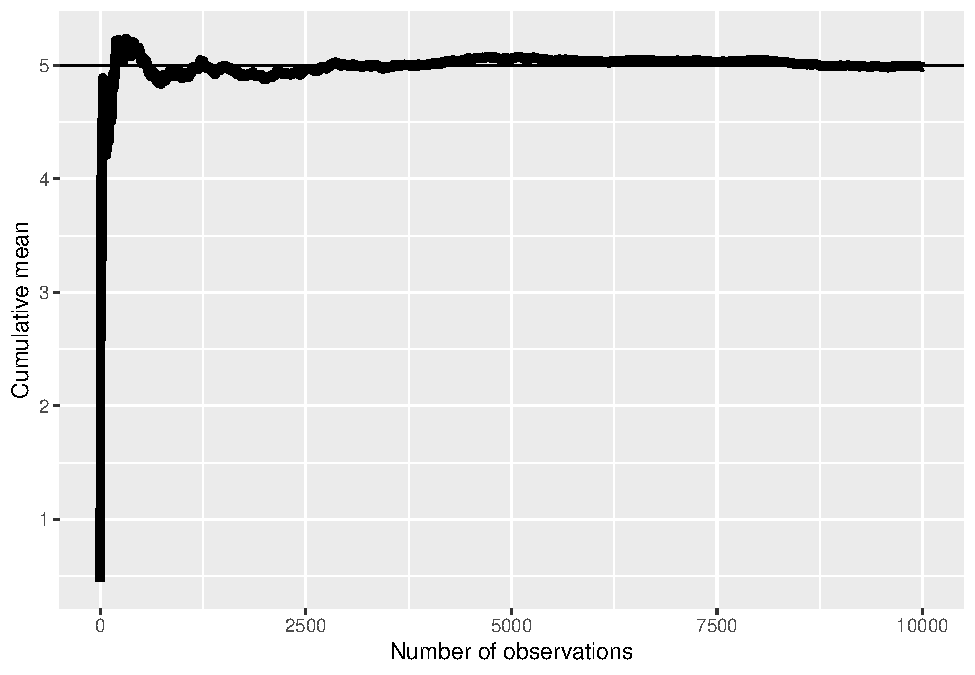
\includegraphics{C6Project_files/figure-latex/cumulativemean-1.pdf}

See how as the number of draws increases, the cumulative mean gets
closer and closer to the true mean, 5. This is a clear demonstration of
the LLN.

\hypertarget{sample-variance-and-theoretical-variance}{%
\subsection{Sample variance and theoretical
variance}\label{sample-variance-and-theoretical-variance}}

We know that the theoretical standard deviation for the exponential
distribution is also 1/lambda = 5. Thus, the variance is simply the
square of the standard deviation, or 25. Let's plot the sample variance
now using the var function.

\begin{Shaded}
\begin{Highlighting}[]
\NormalTok{variance =}\StringTok{ }\KeywordTok{c}\NormalTok{() }\CommentTok{#initialize variance to empty vector}
\ControlFlowTok{for}\NormalTok{(i }\ControlFlowTok{in} \DecValTok{1}\OperatorTok{:}\DecValTok{1000}\NormalTok{) }\CommentTok{#do 1000 simulations}
\NormalTok{  variance =}\StringTok{ }\KeywordTok{c}\NormalTok{(variance, }\KeywordTok{var}\NormalTok{(}\KeywordTok{rexp}\NormalTok{(}\DecValTok{40}\NormalTok{,}\FloatTok{0.2}\NormalTok{))) }\CommentTok{#store the variance of each simulation into the vector}
\KeywordTok{hist}\NormalTok{(variance) }\CommentTok{#plot histogram of variance vector}
\end{Highlighting}
\end{Shaded}

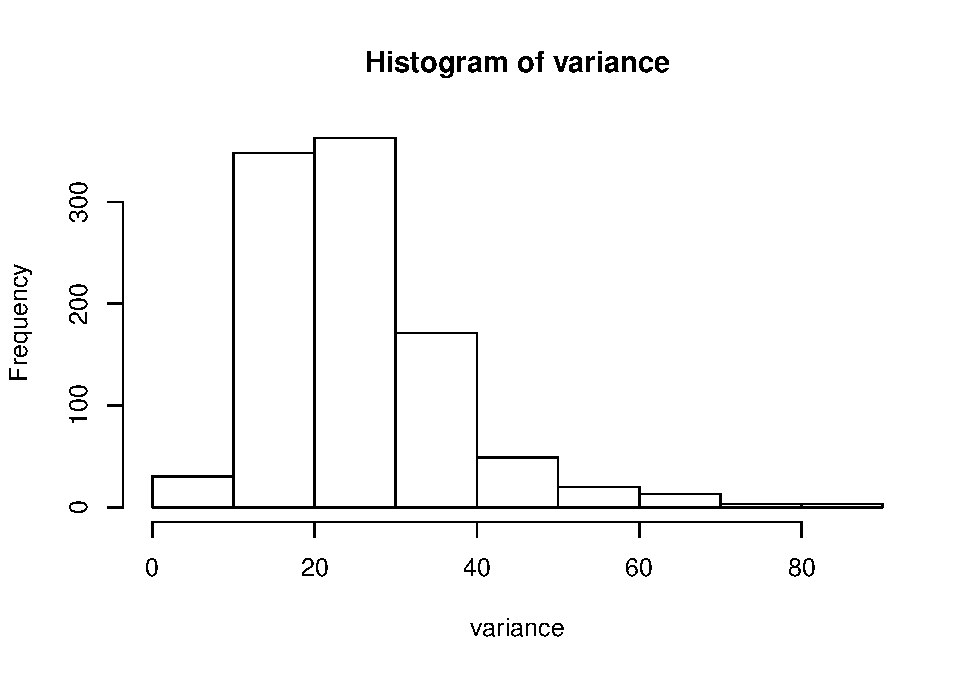
\includegraphics{C6Project_files/figure-latex/variance-1.pdf}

\begin{Shaded}
\begin{Highlighting}[]
\KeywordTok{mean}\NormalTok{(variance) }\CommentTok{#calculate the sample variance}
\end{Highlighting}
\end{Shaded}

\begin{verbatim}
## [1] 25.07948
\end{verbatim}

As we expect, the sample variance is quite close to the theoretical
variance, 25.

\hypertarget{can-we-show-that-the-distribution-is-approximately-normal}{%
\subsection{Can we show that the distribution is approximately
normal?}\label{can-we-show-that-the-distribution-is-approximately-normal}}

At an initial glance, if we just plot a collection of random
exponentials, we would of course see an exponential curve: a higher
volume of low values and a lower volume of high values, forming a steep
curve. Let's take a look right now.

\begin{Shaded}
\begin{Highlighting}[]
\KeywordTok{hist}\NormalTok{(}\KeywordTok{rexp}\NormalTok{(}\DecValTok{1000}\NormalTok{,}\FloatTok{0.2}\NormalTok{))}
\end{Highlighting}
\end{Shaded}

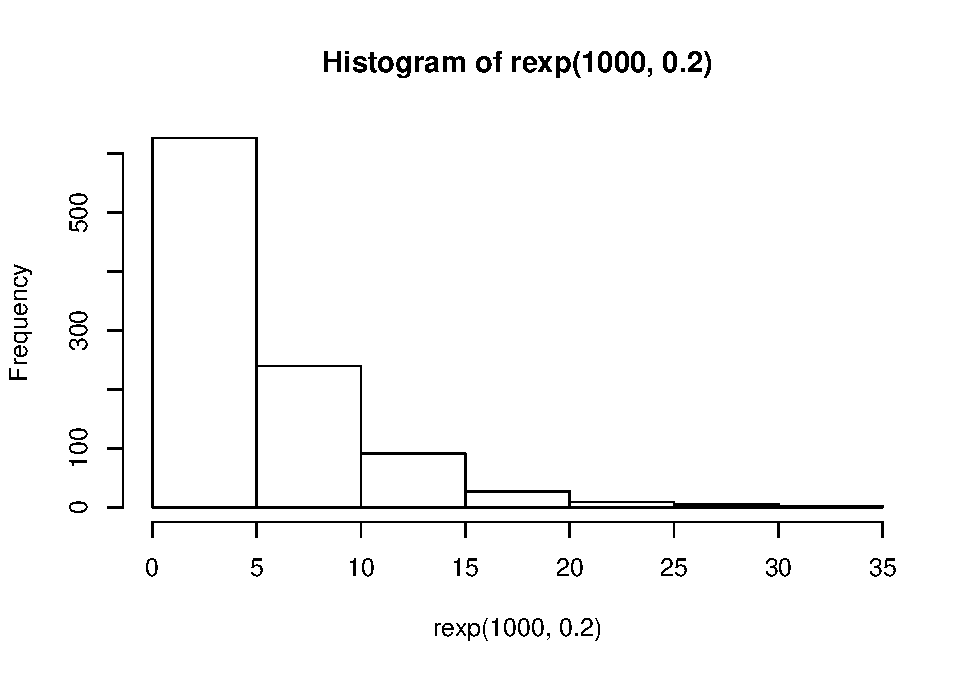
\includegraphics{C6Project_files/figure-latex/exponentialcurve-1.pdf}

Doesn't look very normal, right? Now what about a large collection of
averages of 40 exponentials? Like before, we will run 1000 simulations
of 40 draws from an exponential distribution, then take the average of
each simulation and plot that.

\begin{Shaded}
\begin{Highlighting}[]
\NormalTok{means =}\StringTok{ }\KeywordTok{c}\NormalTok{()}
\ControlFlowTok{for}\NormalTok{ (i }\ControlFlowTok{in} \DecValTok{1}\OperatorTok{:}\DecValTok{1000}\NormalTok{)}
\NormalTok{  means =}\StringTok{ }\KeywordTok{c}\NormalTok{(means, }\KeywordTok{mean}\NormalTok{(}\KeywordTok{rexp}\NormalTok{(}\DecValTok{40}\NormalTok{,}\FloatTok{0.2}\NormalTok{)))}
\NormalTok{mu =}\StringTok{ }\KeywordTok{mean}\NormalTok{(means)}
\NormalTok{s =}\StringTok{ }\KeywordTok{sd}\NormalTok{(means)}
\NormalTok{lines =}\StringTok{ }\KeywordTok{c}\NormalTok{(mu}\DecValTok{-2}\OperatorTok{*}\NormalTok{s,mu}\OperatorTok{-}\NormalTok{s,mu,mu}\OperatorTok{+}\NormalTok{s,mu}\OperatorTok{+}\DecValTok{2}\OperatorTok{*}\NormalTok{s)}
\NormalTok{colors =}\StringTok{ }\KeywordTok{c}\NormalTok{(}\StringTok{"green"}\NormalTok{,}\StringTok{"magenta"}\NormalTok{,}\StringTok{"blue"}\NormalTok{,}\StringTok{"magenta"}\NormalTok{,}\StringTok{"green"}\NormalTok{)}
\NormalTok{g =}\StringTok{ }\KeywordTok{ggplot}\NormalTok{(}\KeywordTok{data.frame}\NormalTok{(means), }\KeywordTok{aes}\NormalTok{(}\DataTypeTok{x =}\NormalTok{ means))}
\NormalTok{g }\OperatorTok{+}\StringTok{ }\KeywordTok{geom_histogram}\NormalTok{(}\DataTypeTok{color =} \StringTok{"red"}\NormalTok{, }\DataTypeTok{fill =} \StringTok{"orange"}\NormalTok{) }\OperatorTok{+}
\StringTok{  }\KeywordTok{geom_vline}\NormalTok{(}\DataTypeTok{xintercept =}\NormalTok{ lines, }\DataTypeTok{linetype =} \StringTok{"dotted"}\NormalTok{, }\DataTypeTok{color =}\NormalTok{ colors, }\DataTypeTok{size =} \FloatTok{1.5}\NormalTok{) }\OperatorTok{+}
\StringTok{  }\KeywordTok{xlab}\NormalTok{(}\StringTok{"Means"}\NormalTok{) }\OperatorTok{+}
\StringTok{  }\KeywordTok{ylab}\NormalTok{(}\StringTok{"Frequency"}\NormalTok{) }\OperatorTok{+}
\StringTok{  }\KeywordTok{ggtitle}\NormalTok{(}\StringTok{"Histogram of 1000 Averages of 40 Exponential Draws"}\NormalTok{)}
\end{Highlighting}
\end{Shaded}

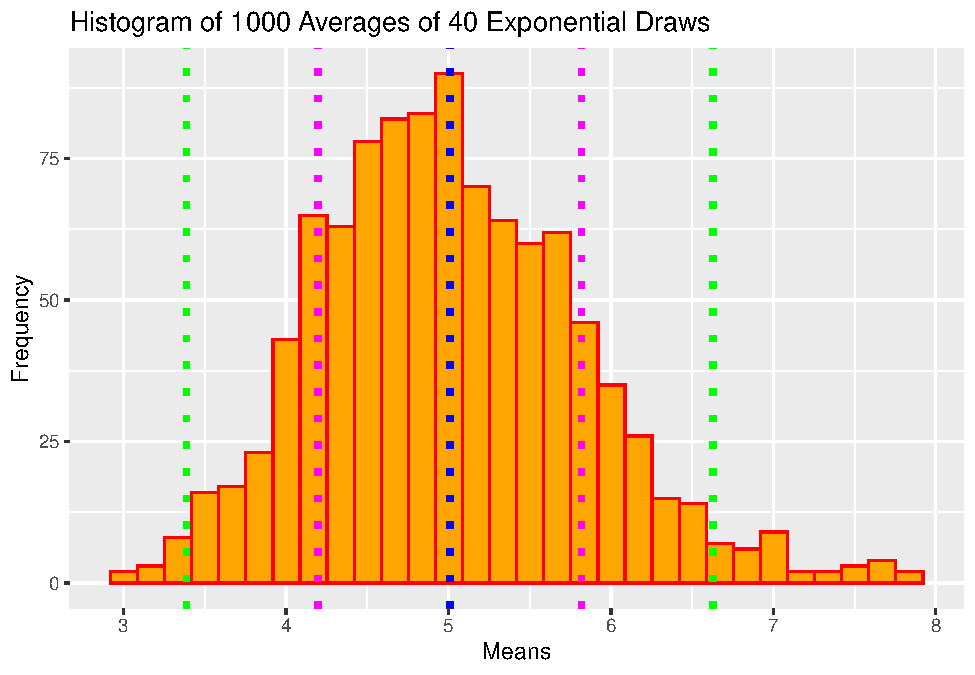
\includegraphics{C6Project_files/figure-latex/normality-1.pdf}

This looks much more normal and approximately centered around the true
mean of the distribution with vertical lines drawn at the mean (blue), 1
standard deviation from the mean (magenta), and 2 standard deviations
from the mean (green). This is due to the Central Limit Theorem, which
states that the distribution of averages of iid variables becomes that
of a standard normal as the sample size increases. So, \(\bar X_n\) is
approximately \(N(\mu, \sigma^2 / n)\) ;

Where \(\mu\) \(\approx\) 5 ; \(\sigma^2\) \(\approx\) 5, and n = 40
such that \(\sigma\) \(\approx\) 5/sqrt(40) \(\approx\) 0.79.

\hypertarget{part-2-inferential-data-analysis}{%
\subsection{Part 2: Inferential Data
Analysis}\label{part-2-inferential-data-analysis}}

The second part of our exploration is to analyze the ToothGrowth dataset
provided in the R datasets package. Let's load this dataset into R and
take a look at what it contains.

\begin{Shaded}
\begin{Highlighting}[]
\KeywordTok{library}\NormalTok{(datasets)}
\KeywordTok{data}\NormalTok{(}\StringTok{"ToothGrowth"}\NormalTok{)}
\NormalTok{TG =}\StringTok{ }\KeywordTok{as_tibble}\NormalTok{(ToothGrowth)}
\KeywordTok{str}\NormalTok{(TG)}
\end{Highlighting}
\end{Shaded}

\begin{verbatim}
## Classes 'tbl_df', 'tbl' and 'data.frame':    60 obs. of  3 variables:
##  $ len : num  4.2 11.5 7.3 5.8 6.4 10 11.2 11.2 5.2 7 ...
##  $ supp: Factor w/ 2 levels "OJ","VC": 2 2 2 2 2 2 2 2 2 2 ...
##  $ dose: num  0.5 0.5 0.5 0.5 0.5 0.5 0.5 0.5 0.5 0.5 ...
\end{verbatim}

The ToothGrowth dataset contains 3 variables: len (numeric), supp
(factor), and dose (numeric). Looking at the R documentation for this
dataset tells us that it contains 60 observations for tooth length,
supplement type, and vitamic C dosage in milligrams/day. The test
subjects were 60 guinea pigs, with certain groups of guinea pigs
receiving varying dosages of vitamin C (0.5,1,and 2 mg/day) and by one
of two delivery methods: orange juice or ascorbic acid. The response
variable here is tooth length, and it is dependent on the dosage levels
of vitamic C given to the pig and the delivery method. Let's take a look
at some of the summary statistics for this dataset, and whether or not
there are any missing values.

\begin{Shaded}
\begin{Highlighting}[]
\KeywordTok{sum}\NormalTok{(}\KeywordTok{is.na}\NormalTok{(TG))}
\end{Highlighting}
\end{Shaded}

\begin{verbatim}
## [1] 0
\end{verbatim}

\begin{Shaded}
\begin{Highlighting}[]
\KeywordTok{summary}\NormalTok{(TG)}
\end{Highlighting}
\end{Shaded}

\begin{verbatim}
##       len        supp         dose      
##  Min.   : 4.20   OJ:30   Min.   :0.500  
##  1st Qu.:13.07   VC:30   1st Qu.:0.500  
##  Median :19.25           Median :1.000  
##  Mean   :18.81           Mean   :1.167  
##  3rd Qu.:25.27           3rd Qu.:2.000  
##  Max.   :33.90           Max.   :2.000
\end{verbatim}

There are no missing values for any of the 60 observations, and it looks
like the base R summary doesn't tell us any more than what we already
know. Since we know that the two predictors, supp and dose, were varied
in order to see their effect on tooth growth, we can try to capture
their effects by grouping. First, let's only group by vitamin C dosage
and compare the tooth growth with each of the 3 dosages. Next, we can
group only by supplement, and compare tooth growth within the two
supplements.

\begin{Shaded}
\begin{Highlighting}[]
\NormalTok{TG_Dose =}\StringTok{ }\NormalTok{TG }\OperatorTok\StringTok{ }\KeywordTok{group_by}\NormalTok{(dose) }\OperatorTok\StringTok{ }\KeywordTok{summarize}\NormalTok{(}\DataTypeTok{mlen =} \KeywordTok{mean}\NormalTok{(len))}
\NormalTok{TG_Dose}
\end{Highlighting}
\end{Shaded}

\begin{verbatim}
## # A tibble: 3 x 2
##    dose  mlen
##   <dbl> <dbl>
## 1   0.5  10.6
## 2   1    19.7
## 3   2    26.1
\end{verbatim}

\begin{Shaded}
\begin{Highlighting}[]
\NormalTok{TG}\OperatorTok{$}\NormalTok{dose =}\StringTok{ }\KeywordTok{as.factor}\NormalTok{(TG}\OperatorTok{$}\NormalTok{dose)}
\NormalTok{g =}\StringTok{ }\KeywordTok{ggplot}\NormalTok{(TG, }\KeywordTok{aes}\NormalTok{(}\DataTypeTok{x =}\NormalTok{ dose, }\DataTypeTok{y =}\NormalTok{ len, }\DataTypeTok{color =}\NormalTok{ dose))}
\NormalTok{g }\OperatorTok{+}\StringTok{ }\KeywordTok{geom_boxplot}\NormalTok{(}\DataTypeTok{fill =} \StringTok{"yellow"}\NormalTok{) }\OperatorTok{+}
\StringTok{  }\KeywordTok{xlab}\NormalTok{(}\StringTok{"Vitamin C Dosage"}\NormalTok{) }\OperatorTok{+}
\StringTok{  }\KeywordTok{ylab}\NormalTok{(}\StringTok{"Average Tooth Length"}\NormalTok{) }\OperatorTok{+}
\StringTok{  }\KeywordTok{ggtitle}\NormalTok{(}\StringTok{"Average Tooth Length by Vitamin C Dosage"}\NormalTok{)}
\end{Highlighting}
\end{Shaded}

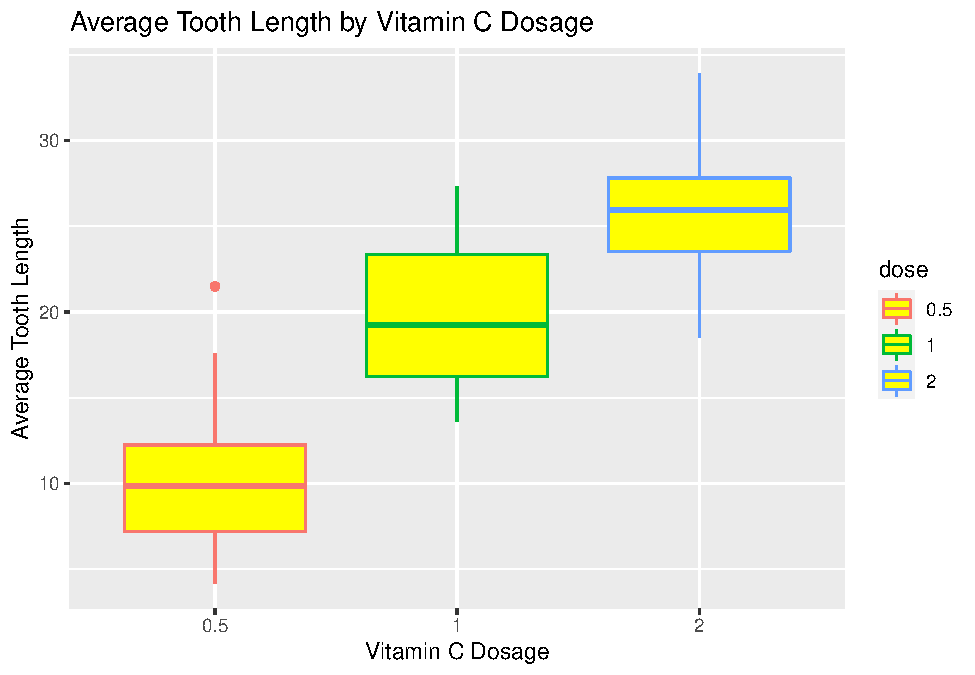
\includegraphics{C6Project_files/figure-latex/groupdose-1.pdf}

What we find after grouping each observation together based on dosage is
that there appears to be a clear positive relationship between guinea
pig tooth length and vitamin C dosage. Since there are 3 groups, we can
provide evidence for this relationship by constructing 95\% confidence
intervals for the difference in mean tooth length of each group and
doing two-sample t tests. If the confidence intervals do not contain 0,
then there is very strong evidence that the means between groups are not
equal. Furthermore, the test statistic and p-value would also tell us
that we would reject the null hypothesis \(\mu1\) = \(\mu2\). This will
be done by comparing the means of tooth length given doses 0.5 and 1,
and then the means given doses 1 and 2.

In the first test, our null hypothesis is that the mean(len\textbar dose
= 0.5) is equal to the mean(len\textbar dose = 1). We begin by creating
a subset of the ToothGrowth dataset which contains only observations
where dosage = 0.5 or dosage = 1. Then, we perform a t.test using paired
= FALSE. The reason for this is that there is no logic behind pairing
pigs that received a 0.5mg dose of vitamin C with pigs that received a
1mg dose of vitamin C, since different pigs were used for each
observation. It turns out the confidence interval remains unchanged
whether var.equal is set to TRUE or FALSE, so we don't have to specify
that parameter. We do a two-sided t test because if we reject, then by
default we also reject the one-sided test.

\begin{Shaded}
\begin{Highlighting}[]
\NormalTok{dose12 =}\StringTok{ }\KeywordTok{subset}\NormalTok{(TG, dose }\OperatorTok{==}\StringTok{ }\FloatTok{0.5} \OperatorTok{|}\StringTok{ }\NormalTok{dose }\OperatorTok{==}\StringTok{ }\DecValTok{1}\NormalTok{)}
\KeywordTok{t.test}\NormalTok{(len }\OperatorTok{~}\StringTok{ }\NormalTok{dose, }\DataTypeTok{paired =} \OtherTok{FALSE}\NormalTok{, }\DataTypeTok{alternative =} \StringTok{"two.sided"}\NormalTok{, }\DataTypeTok{data =}\NormalTok{ dose12)}
\end{Highlighting}
\end{Shaded}

\begin{verbatim}
## 
##  Welch Two Sample t-test
## 
## data:  len by dose
## t = -6.4766, df = 37.986, p-value = 1.268e-07
## alternative hypothesis: true difference in means is not equal to 0
## 95 percent confidence interval:
##  -11.983781  -6.276219
## sample estimates:
## mean in group 0.5   mean in group 1 
##            10.605            19.735
\end{verbatim}

The test statistic is -6.4766 and the p-value is extremely small, so we
very clearly reject the null hypothesis that the difference in means is
0. Looking at the confidence interval, we can see the practical side of
rejecting the null and observe that the difference between
mean(len\textbar dose = 1) and mean(len\textbar dose = 0.5) is within
that interval with 95\% confidence.

In the next test, our null hypothesis is that the mean(len\textbar dose
= 1) is equal to the mean(len\textbar dose = 2). We follow exactly the
same steps as before, except we subset out observations where dosage = 1
and dosage = 2. We perform the t test and examine the results.

\begin{Shaded}
\begin{Highlighting}[]
\NormalTok{dose23 =}\StringTok{ }\KeywordTok{subset}\NormalTok{(TG, dose }\OperatorTok{==}\StringTok{ }\DecValTok{1} \OperatorTok{|}\StringTok{ }\NormalTok{dose }\OperatorTok{==}\StringTok{ }\DecValTok{2}\NormalTok{)}
\KeywordTok{t.test}\NormalTok{(len }\OperatorTok{~}\StringTok{ }\NormalTok{dose, }\DataTypeTok{paired =} \OtherTok{FALSE}\NormalTok{, }\DataTypeTok{alternative =} \StringTok{"two.sided"}\NormalTok{, }\DataTypeTok{data =}\NormalTok{ dose23)}
\end{Highlighting}
\end{Shaded}

\begin{verbatim}
## 
##  Welch Two Sample t-test
## 
## data:  len by dose
## t = -4.9005, df = 37.101, p-value = 1.906e-05
## alternative hypothesis: true difference in means is not equal to 0
## 95 percent confidence interval:
##  -8.996481 -3.733519
## sample estimates:
## mean in group 1 mean in group 2 
##          19.735          26.100
\end{verbatim}

Once again, we reject the null because our t-statistic is less than the
alpha = 0.05 t quantile, and the p-value is less than 0.05. It also
follows that we would reject for the null hypothesis
mean(len\textbar dose = 0.5) = mean(len\}dose = 2) for obvious reasons.

Now let's look at what happens to the mean tooth length when we group by
supp.

\begin{Shaded}
\begin{Highlighting}[]
\NormalTok{TG_Supp =}\StringTok{ }\NormalTok{TG }\OperatorTok\StringTok{ }\KeywordTok{group_by}\NormalTok{(supp) }\OperatorTok\StringTok{ }\KeywordTok{summarize}\NormalTok{(}\DataTypeTok{mlen =} \KeywordTok{mean}\NormalTok{(len))}
\NormalTok{TG_Supp}
\end{Highlighting}
\end{Shaded}

\begin{verbatim}
## # A tibble: 2 x 2
##   supp   mlen
##   <fct> <dbl>
## 1 OJ     20.7
## 2 VC     17.0
\end{verbatim}

\begin{Shaded}
\begin{Highlighting}[]
\NormalTok{g =}\StringTok{ }\KeywordTok{ggplot}\NormalTok{(TG, }\KeywordTok{aes}\NormalTok{(}\DataTypeTok{x =}\NormalTok{ supp, }\DataTypeTok{y =}\NormalTok{ len, }\DataTypeTok{color =}\NormalTok{ supp))}
\NormalTok{g }\OperatorTok{+}\StringTok{ }\KeywordTok{geom_dotplot}\NormalTok{(}\DataTypeTok{binaxis =} \StringTok{"y"}\NormalTok{, }\DataTypeTok{stackdir =} \StringTok{"center"}\NormalTok{) }\OperatorTok{+}
\StringTok{  }\KeywordTok{xlab}\NormalTok{(}\StringTok{"Supplement Type"}\NormalTok{) }\OperatorTok{+}
\StringTok{  }\KeywordTok{ylab}\NormalTok{(}\StringTok{"Average Tooth Length"}\NormalTok{) }\OperatorTok{+}
\StringTok{  }\KeywordTok{ggtitle}\NormalTok{(}\StringTok{"Average Tooth Length by Supplement"}\NormalTok{)}
\end{Highlighting}
\end{Shaded}

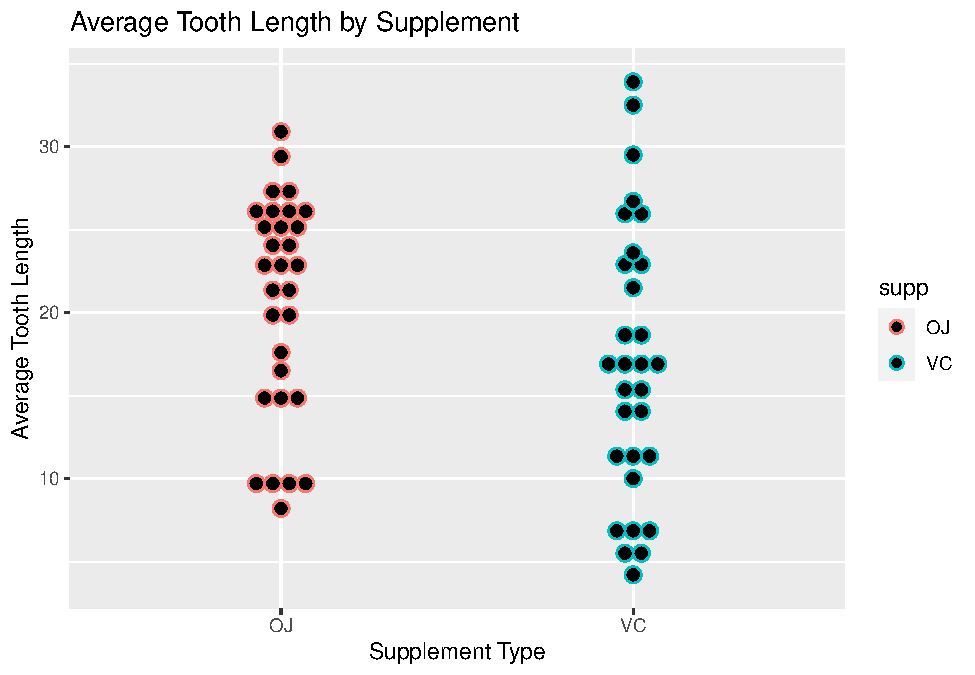
\includegraphics{C6Project_files/figure-latex/groupsupp-1.pdf}

Looks like there is a slight difference in mean tooth length for pigs
receiving orange juice versus ascorbic acid. Again, we define our null
hypothesis to be mean(len\textbar supp=OJ) = mean(len\textbar supp=VC)
and the alternative is that the difference is less than 0. Then we use
t.test specifying supp as the explanatory variable of interest. Since
there are only two levels in supp, we do not have to do any subsetting.

\begin{Shaded}
\begin{Highlighting}[]
\KeywordTok{t.test}\NormalTok{(len }\OperatorTok{~}\StringTok{ }\NormalTok{supp, }\DataTypeTok{paired =} \OtherTok{FALSE}\NormalTok{, }\DataTypeTok{alternative =} \StringTok{"two.sided"}\NormalTok{, }\DataTypeTok{data =}\NormalTok{ TG)}
\end{Highlighting}
\end{Shaded}

\begin{verbatim}
## 
##  Welch Two Sample t-test
## 
## data:  len by supp
## t = 1.9153, df = 55.309, p-value = 0.06063
## alternative hypothesis: true difference in means is not equal to 0
## 95 percent confidence interval:
##  -0.1710156  7.5710156
## sample estimates:
## mean in group OJ mean in group VC 
##         20.66333         16.96333
\end{verbatim}

What we find is that with alpha = 0.05, we actually fail to reject the
null hypothesis, because the p-value is \textgreater{} 0.05 and the
confidence interval contains zero. However, note how close the p-value
is to 0.05 and how the confidence interval barely contains zero. What
might happen if we decide to do a one-sided test instead?

\begin{Shaded}
\begin{Highlighting}[]
\KeywordTok{t.test}\NormalTok{(len }\OperatorTok{~}\StringTok{ }\NormalTok{supp, }\DataTypeTok{paired =} \OtherTok{FALSE}\NormalTok{, }\DataTypeTok{alternative =} \StringTok{"greater"}\NormalTok{, }\DataTypeTok{data =}\NormalTok{ TG)}
\end{Highlighting}
\end{Shaded}

\begin{verbatim}
## 
##  Welch Two Sample t-test
## 
## data:  len by supp
## t = 1.9153, df = 55.309, p-value = 0.03032
## alternative hypothesis: true difference in means is greater than 0
## 95 percent confidence interval:
##  0.4682687       Inf
## sample estimates:
## mean in group OJ mean in group VC 
##         20.66333         16.96333
\end{verbatim}

Interestingly enough, now we do reject the null hypothesis, because the
p-value is \textless{} 0.05 and the CI does not contain zero. Thus, we
are in favor of the alternative that the difference in means is greater
than zero.

\hypertarget{conclusions-and-assumptions-needed}{%
\subsection{Conclusions and Assumptions
Needed}\label{conclusions-and-assumptions-needed}}

Based on the results of the t tests conducted, we conclude that greater
dosages of vitamin C result in greater tooth lengths in guinea pigs. We
also conclude that orange juice as a delivery method as opposed to
ascorbic acid results in greater tooth lengths on average. For these
conclusions to hold, we must assume that the data collected in this
dataset were iid, and that the sample size is large enough that the t
distribution becomes approximately standard normal.

\end{document}
